\documentclass{article}%
\usepackage{amsmath}%
\usepackage{amsfonts}%
\usepackage{amssymb}%
\usepackage{graphicx}
%-------------------------------------------
\newtheorem{theorem}{Theorem}
\newtheorem{acknowledgement}[theorem]{Acknowledgement}
\newtheorem{algorithm}[theorem]{Algorithm}
\newtheorem{axiom}[theorem]{Axiom}
\newtheorem{case}[theorem]{Case}
\newtheorem{claim}[theorem]{Claim}
\newtheorem{conclusion}[theorem]{Conclusion}
\newtheorem{condition}[theorem]{Condition}
\newtheorem{conjecture}[theorem]{Conjecture}
\newtheorem{corollary}[theorem]{Corollary}
\newtheorem{criterion}[theorem]{Criterion}
\newtheorem{definition}[theorem]{Definition}
\newtheorem{example}[theorem]{Example}
\newtheorem{exercise}[theorem]{Exercise}
\newtheorem{lemma}[theorem]{Lemma}
\newtheorem{notation}[theorem]{Notation}
\newtheorem{problem}[theorem]{Problem}
\newtheorem{proposition}[theorem]{Proposition}
\newtheorem{remark}[theorem]{Remark}
\newtheorem{solution}[theorem]{Solution}
\newtheorem{summary}[theorem]{Summary}
\newenvironment{proof}[1][Proof]{\textbf{#1.} }{\ \rule{0.5em}{0.5em}}
\setlength{\textwidth}{7.0in}
\setlength{\oddsidemargin}{-0.35in}
\setlength{\topmargin}{-0.5in}
\setlength{\textheight}{9.0in}
\setlength{\parindent}{0.3in}
\begin{document}

\begin{flushright}
\textbf{Ziad Arafat \\
FEB 10, 2017}
\end{flushright}

\begin{center}
\textbf{CS 111: CS Principles \\
Homework III} \\
\end{center}

\section*{P.139 Q2}
\subsection*{a.}
\begin{enumerate}
\item Set $a$ to 12.
\item Set $b$ to $a+1$.
\item Set $c$ to $b \times a \div 12$.
\item Print the value of $c$
\end{enumerate}

\subsection*{b.}
$78$

\section*{P.140 Q3}

\subsection*{a.}
\begin{enumerate}
\item Set F to a list [1, 1]
\item Set x to 1 and y to 2
\item Set z to 1
\item While z is less than or equal to 20:
\begin{enumerate}
\item Append the sum of F[x] and F[y] to the end of list F
\item Increment x, y, and z by 1
\end{enumerate}
\item End of loop
\item Print the value of F[20]
\end{enumerate}\textbf{•}

\newpage

\subsection*{b.}
$6765$

\subsection*{c.}
I think the the recursive algorithm is more efficient simply because it's easier to implement and because it ends up being less steps than calculating the equation. It is also much simpler to understand and rings more with the fibonacci sequence. However once we approach bigger numbers it becomes clear that the equation is much more efficient because it then involves much less steps so if we were to compute F[100] I would say the equation is better over all. 
\newpage1
\subsection*{d.}
Done in Python
\newline
\begin{center}
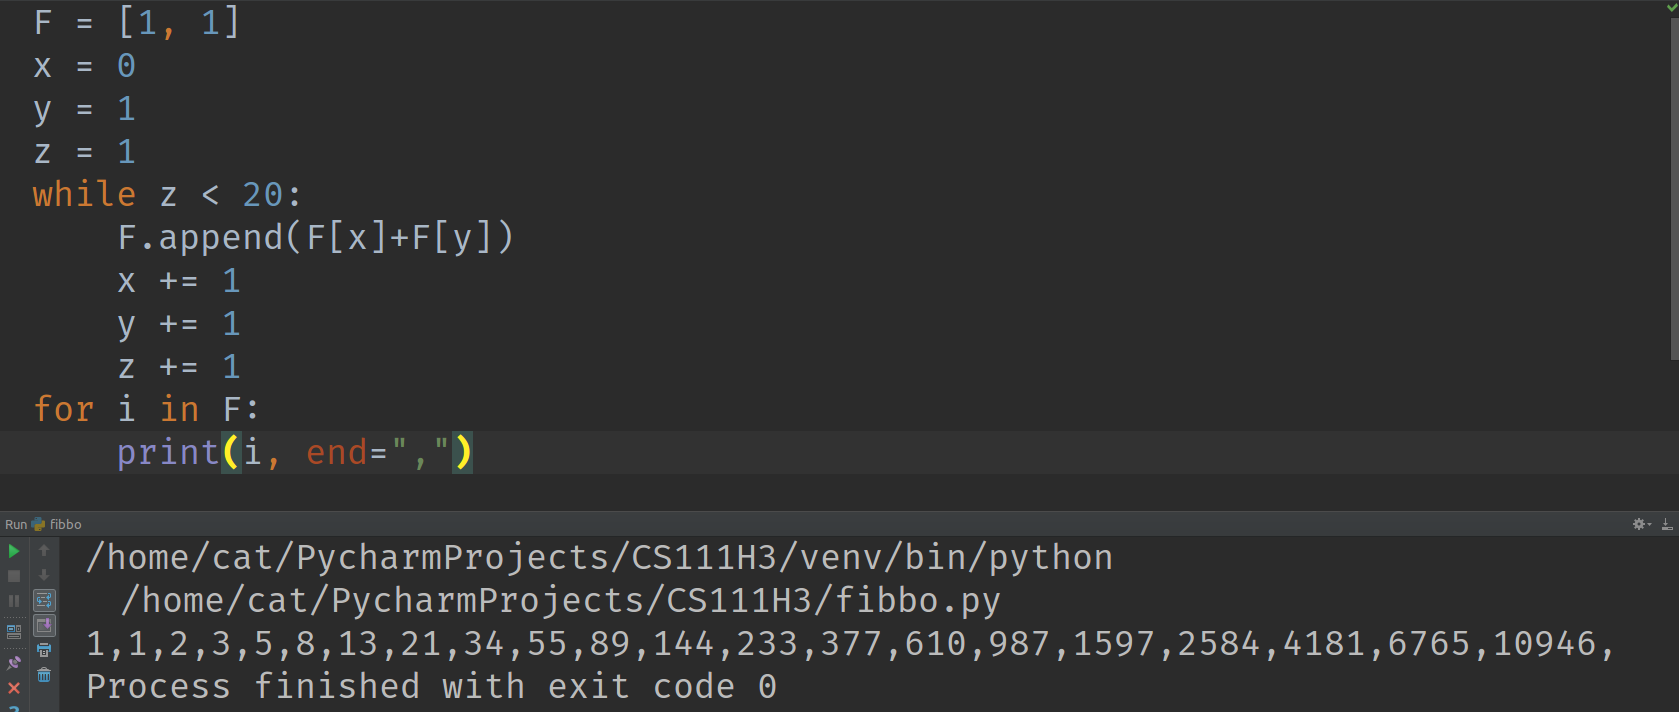
\includegraphics[scale=0.3]{/home/cat/Documents/notes/CS111/Pycharm1.png}
\end{center}


\subsection*{e.}
Here is code using the iterative algorithm \newline
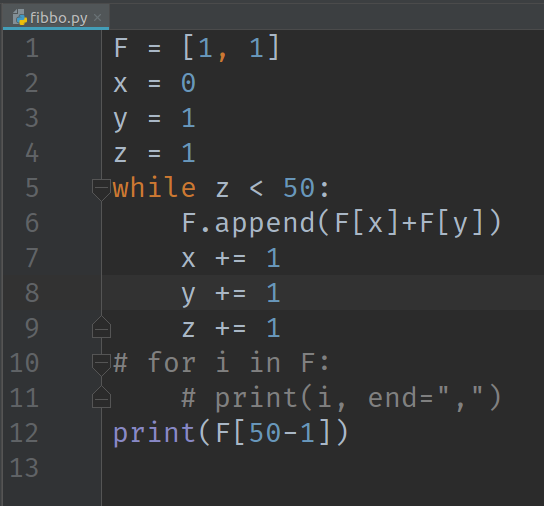
\includegraphics[scale=0.3]{/home/cat/Documents/notes/CS111/fibbo.png}

code using the recursive calculation in Python's default math library \newline
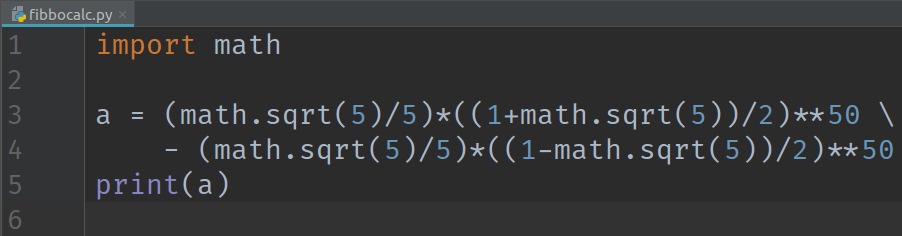
\includegraphics[scale=0.3]{/home/cat/Documents/notes/CS111/fibbocalc.png}
\newpage

\newpage
\section*{P.141 Q7}
\subsection*{a.}
linear/sequential search takes $n$ comparisons in worst case and $1$ comparison in best case. So the average is $\Theta(\frac{n}{2})$. $(32million \div 2)\div 12000 = 1333seconds = 12minutes\ 13seconds$

\subsection*{b.}
The average case of binary search is $\Theta(\log_2 n)$. So $\log_2 32million \div 12000 \approx 0.002s \approx 2ms$

\section*{P.141 Q8}
\subsection*{a.}
It appears you will need at least or more than 14 pancakes for the algorithm's use to make any sense.

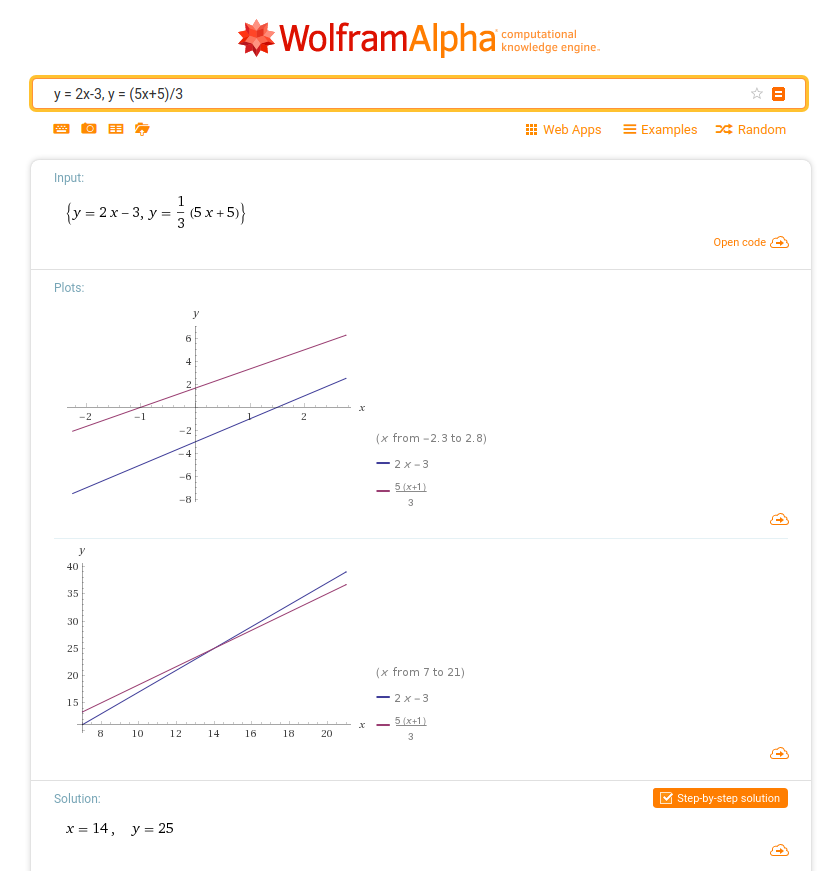
\includegraphics[scale=0.5]{/home/cat/Documents/notes/CS111/Wolfram1.png}

\clearpage
\section*{P.141-142 Q11}
\subsection*{a.}

\noindent \textbf{Bubble Sort}

4, 8, 2, 6, 

4, 2, 6, 8

2, 4, 6, 8

\noindent \textbf{Selection Sort}

4, 8, 2, 6, 

2, 8, 4, 6, 

2, 4, 8, 6, 

2, 4, 6, 8, \newline \newline

\subsection*{b.}
\noindent \textbf{Bubble Sort}

12, 3, 6, 8, 2, 5, 7, 

3, 6, 8, 2, 5, 7, 12, 

3, 6, 2, 5, 7, 8, 12, 

3, 2, 5, 6, 7, 8, 12, 

2, 3, 5, 6, 7, 8, 12, 

\noindent \textbf{Selection Sort}

12, 3, 6, 8, 2, 5, 7, 

2, 3, 6, 8, 12, 5, 7, 

2, 3, 5, 8, 12, 6, 7, 

2, 3, 5, 6, 12, 8, 7, 

2, 3, 5, 6, 7, 8, 12, 


\subsection*{c.}
\noindent \textbf{Bubble Sort}

D, B, G, F, A, C, E, H,

B, D, F, A, C, E, G, H,

B, D, A, C, E, F, G, H,
 
B, A, C, D, E, F, G, H,

A, B, C, D, E, F, G, H,

\noindent \textbf{Selection Sort}

D, B, G, F, A, C, E, H,

A, B, G, F, D, C, E, H,

A, B, C, F, D, G, E, H,

A, B, C, D, F, G, E, H,

A, B, C, D, E, G, F, H,

A, B, C, D, E, F, G, H,

\clearpage
\vspace*{0.5in}
\noindent Done in LaTeX
\end{document}